\documentclass[10pt,a4paper,twoside,openright,titlepage]{book}
\usepackage{pifont}
\usepackage{keyval}
\usepackage{color}
\usepackage{fancybox}
\usepackage{amssymb}
\usepackage{amsmath}
\usepackage{graphicx}
\usepackage[colorlinks=true,linkcolor=black,urlcolor=blue,citecolor=black]{hyperref}
\usepackage{calc}
\usepackage{fancyhdr}
\usepackage[inner=5cm,outer=2cm,ignoreheadfoot,top=4cm,bottom=5cm,footskip=4cm]{geometry}
\usepackage{marvosym}
\usepackage{tocloft}
\usepackage{textcomp}
\usepackage{makeidx}
\usepackage{listings}
\usepackage[framed]{mcode}
\usepackage{setspace}
\usepackage{fancyvrb}
\usepackage[]{caption}
\usepackage{lscape}
\usepackage{tabularx}
\usepackage{eso-pic}
\usepackage{rotating}
\usepackage{natbib}
\usepackage{needspace}




\definecolor{orange}{rgb}{1,0.5,0}
\definecolor{mkeywordcolor}{rgb}{0,0,1}
\definecolor{mstringcolor}{rgb}{0.6275,0.1255,0.9412}
\definecolor{mcommentcolor}{rgb}{0,0.5,0}
\definecolor{dkgreen}{rgb}{0,0.6,0}
\definecolor{gray}{rgb}{0.5,0.5,0.5}
\definecolor{lgray}{rgb}{0.85,0.85,0.85}

\setlength{\captionmargin}{3.25cm}
\setlength\parindent{0pt}
\setlength{\parskip}{0.75em}
\setlength{\skip\footins}{2cm}
%\setlength\footbibskip{1cm}

\linespread{1}

\makeindex


%\citestyle{egu}

\renewcommand{\arraystretch}{1.5}

\pagestyle{fancy}
\fancyhf{} % clear all header and footer fields
\renewcommand{\headrulewidth}{0pt}
\renewcommand{\headrulewidth}{0pt}
\fancyfoot[OC,EC]{--\ \thepage{}\ --}


\hyphenation{cali-brate re-pre-sen-ta-tion sub-surface qua-lity pro-cedure
hydro-geo-chemi-cal hydro-metric know-ledge levels Horton para-meter thres-hold
hydro-logy hill-slope capa-city accor-ding satu-ration du-ring element
experi-ment experi-ments using model models distri-buted Nash Sutcliffe
hydro-phobicity hydro-logical homo-geneous hetero-geneous hetero-geneously
homo-geneity hetero-geneity macro-pore hydro-logic up-slope tracer tracers
speci-fied areas cali-bration easily beha-vior array MATLAB sensor matrices
before creates colors color color-map residual priori posteriori auto-matic
propa-gated parent}


% % % % % % % % % % % % % % % % % % % % % % % % % % % % % % % % % % % %
% exercises that we would like people to do:
\newcounter{smallqcounter}
\setcounter{smallqcounter}{0}
\newcommand{\smallq}[1]{
\begin{list}{$\blacktriangleright$ \arabic{smallqcounter}.}
{
\setlength\labelwidth{3cm}
\setlength{\topsep}{0em}
\setlength{\leftmargin}{0cm}
\stepcounter{smallqcounter}
}
\item{#1}
\end{list}
}
% % % % % % % % % % % % % % % % % % % % % % % % % % % % % % % % % % % %

% % % % % % % % % % % % % % % % % % % % % % % % % % % % % % % % % % % %
% optional exercises:
\newcommand{\smallqo}[1]{
\begin{list}{$\vartriangleright$ \arabic{smallqcounter}.}
{
\setlength\labelwidth{3cm}
\setlength{\topsep}{0em}
\setlength{\leftmargin}{0cm}
\stepcounter{smallqcounter}
}
\item{#1}
\end{list}
}
% % % % % % % % % % % % % % % % % % % % % % % % % % % % % % % % % % % %









\sloppy
\newcommand{\guitext}[1]{``\textsf{#1}''}
\newcommand{\MATLAB}[0]{\textsc{MATLAB}}
\newcommand{\starred}[1]{$\ast{}$\textit{#1}$\ast{}$}

\newcommand{\prompt}[1]{\vspace{0.25em}\par\noindent{\tt \textgreater\textgreater\ #1}\vspace{0.25em}\par}

\newcommand{\hintbox}[1]{\noindent
\begin{minipage}[0]{\textwidth}{\vspace{2em} \centering \begin{minipage}[0]{0.6\textwidth}{\hrule \vspace{0.5em}\textsc{\textbf{TIP:\,}} \small #1\vspace{0.5em}
\hrule }\end{minipage} \vspace{2em} \end{minipage}}
}%hintbox


\setlength\fboxsep{0pt}
\setlength\fboxrule{0.2pt}





\newcommand{\squote}[1]{\textquotesingle #1\textquotesingle } % 39 is the decimal ascii code for single straight quote.

\renewcommand{\captionfont}{\footnotesize}
\renewcommand{\captionlabelfont}{\sffamily}


\title{SCGE-2011 Summer course Computational Geo-Ecology -- Inverse modeling}

\author{Willem Bouten \\ Jasper A. Vrugt \\ Sander Huisman \\ Jurriaan H. Spaaks}

\lstset{language=Matlab,
   keywords={break,case,catch,continue,else,elseif,end,for,function,      global,if,otherwise,persistent,return,switch,try,while},
    morekeywords={...},
   alsoletter={...},
   basicstyle=\scriptsize\ttfamily,
   keywordstyle=\color{mkeywordcolor},
   commentstyle=\color{mcommentcolor},
   stringstyle=\color{mstringcolor},
   numbers=left,
   numberstyle=\scriptsize\ttfamily{\color{gray}},
   stepnumber=1,
   numbersep=3mm,
   backgroundcolor=\color{lgray},
   tabsize=4,
   showspaces=false,
   showstringspaces=false,
   frame=none,
   framexleftmargin=2mm,
   aboveskip = 0.5em,
   belowskip = 0.5em,
   xleftmargin = 2mm,
}
\renewcommand{\lstlistingname}{Code Snippet}

\newcommand{\insertemptypage}[0]{
    \vfill
    \newpage
    \thispagestyle{empty}
    \mbox{}
    \pagebreak
}


\begin{document}

\begin{titlepage}
\thispagestyle{empty}


\AddToShipoutPicture*{%
\put(0,0){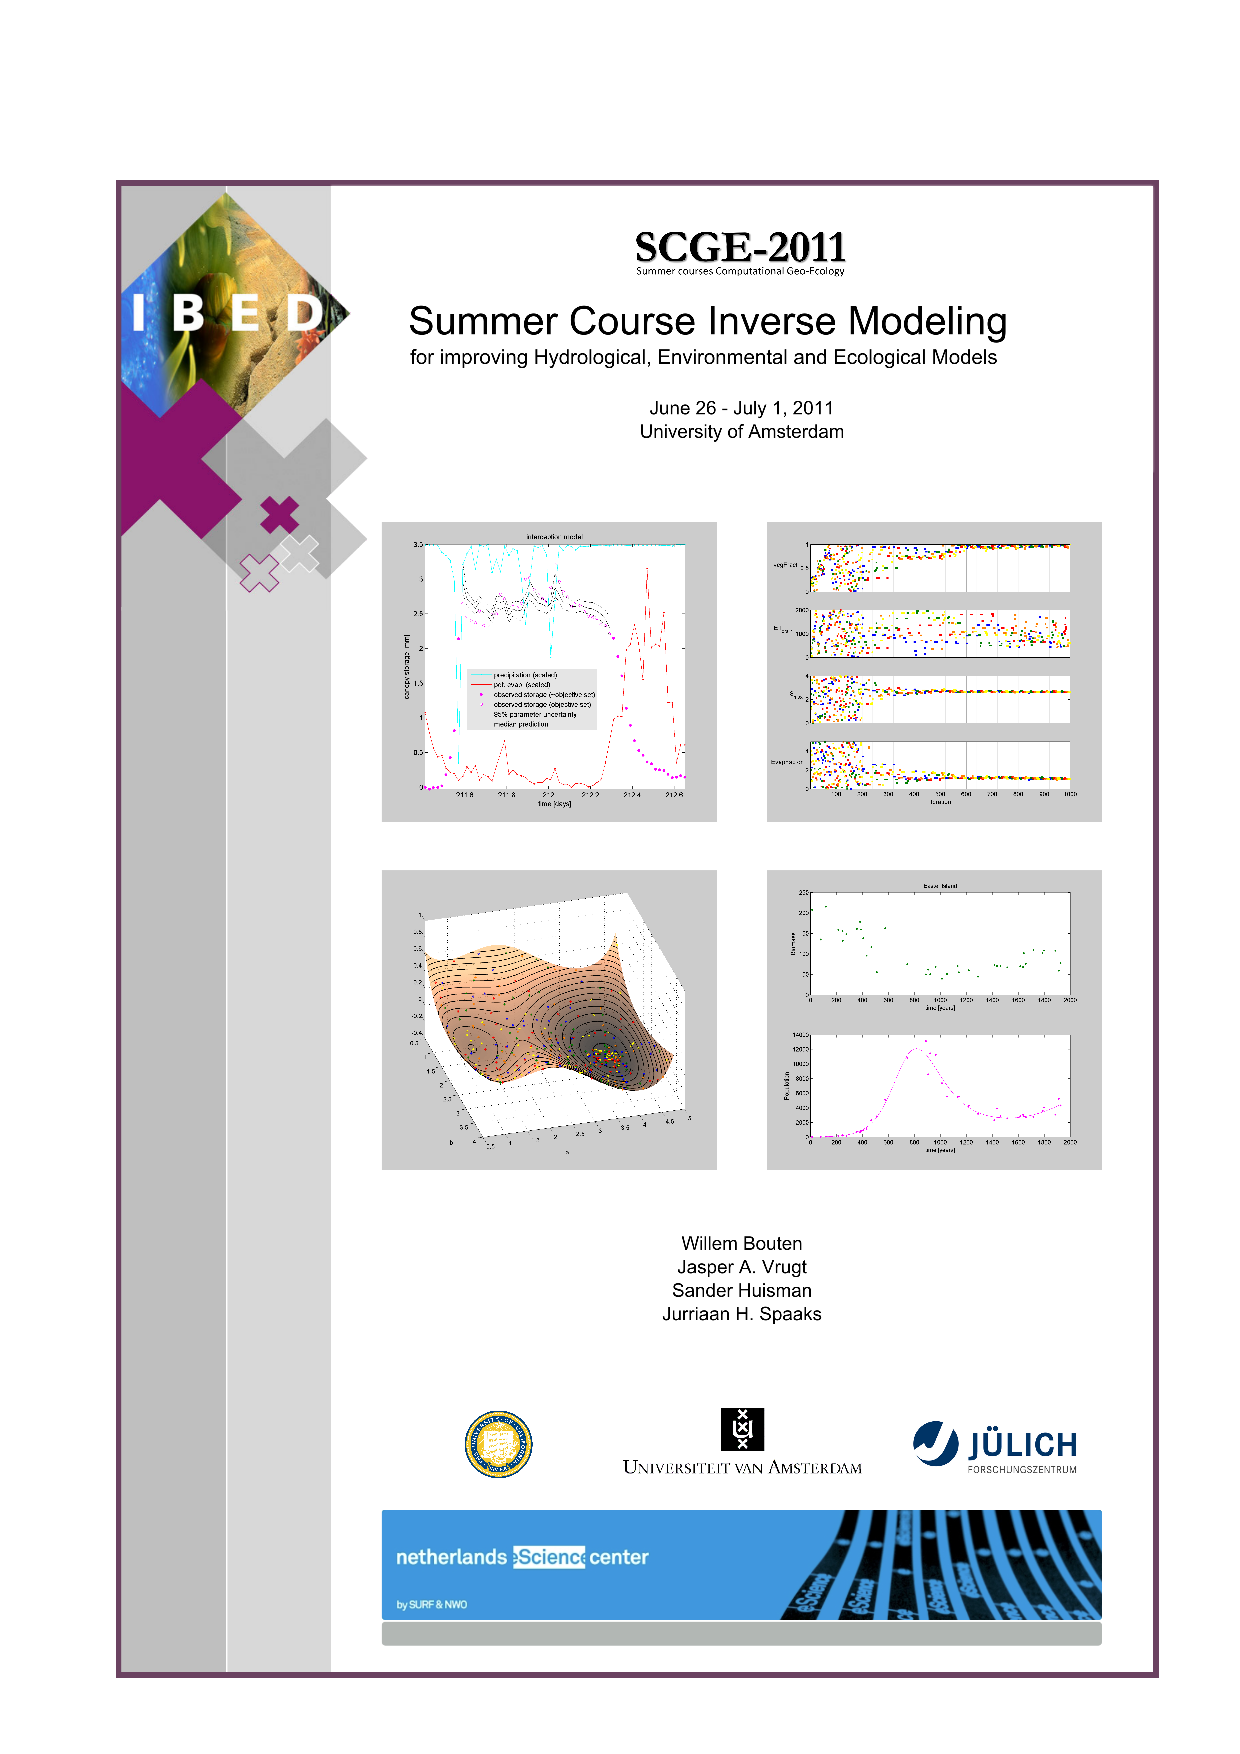
\includegraphics{./eps/converted/syllabus-front}}%
}

\end{titlepage}

\insertemptypage{}
\insertemptypage{}

\frontmatter
%\clearpage\mbox{}\clearpage

\tableofcontents
\newpage

\mainmatter
\chapter{Introduction}
\thispagestyle{fancy}
\label{ch:introduction}


Dear participant, welcome to the SCGE summer course on Inverse Modeling. The document you have before you contains all of the exercises you will be making as part of the course. There are two types of exercise, labeled differently:

\smallq{The exercises indicated by a black solid triangle are the core exercises; most of these will be discussed in class. Any files needed for completing the exercises can be found in the appropriate subdirectory of `./exercises/'. Solutions are also available for most exercises; these are stored under `./solutions/'. As you can see, the exercises are numbered for convenient referencing.}

\smallqo{The exercises indicated by an open triangle are optional exercises; these, you can make if the topic has your specific interest or if you feel you could use some more training, or just for fun!}

Feel free to ask any of us if something isn't clear. You are also encouraged to discuss your results with the other participants. We hope you'll enjoy the course!



\setcounter{smallqcounter}{0}





\chapter{Program}
\thispagestyle{fancy}
\label{ch:program}



\begin{itemize}
\scriptsize
\item[]{Sunday 26/06}
\begin{itemize}
\item{Get-together and dinner at Ponteneur (from 17:30 onward)}
\end{itemize}
\item[]{Monday 27/06: Getting started}
\begin{itemize}
\item{Welcome \& Program of the week}
\item{Introduction to inverse modeling (lecture Willem)}
\item{Local search methodologies (lecture Sander and exercises)}
\item{12.00--13.00: for those who are interested, there's a lecture by Simon Levin ``Evolution of ecosystem properties'' in room C.0.110}
\item{Local \textit{vs.} global search (lecture Jasper)}
\item{Implementing a simple global optimization algorithm (exercises)}
\end{itemize}
 % % % % % % % % % % % % % % % % % % % % % % % % % % % % % % % % % % % % % % % %
\item[]{Tuesday 28/06: Working with DREAM}
\begin{itemize}
\item{Uncertainty of model output and parameter estimates (lecture Jasper)}
\item{DREAM toolbox (exercises)}
\item{Implementing a new model (exercises)}
\end{itemize}
 % % % % % % % % % % % % % % % % % % % % % % % % % % % % % % % % % % % % % % % %
\item[]{Wednesday 29/06: Objectives \& Information in Data}%
\begin{itemize}
\item{Introduction to exercises (lecture Willem)}
\item{Distribution of information within the data (exercises)}
\item{Data transformation (exercises)}
\item{Multi-objective optimization (lecture Jasper)}
\item{Model complexity \textit{vs.} information content of data (exercises)}
\item{Final discussion with questions}
\end{itemize}
 % % % % % % % % % % % % % % % % % % % % % % % % % % % % % % % % % % % % % % % %
\item[]{Thursday 30/06: Analysis of model-observation discrepancies}
\begin{itemize}
\item{Opportunity to answer questions that have come up during the week}
\item{Combining data assimilation and parameter identification (lectures Willem, Jasper, Jurriaan)}
\item{Inverse modeling on parallel machines (lectures Pieter, Jasper)}
\item{Planning of activities on Friday}
\end{itemize}
 % % % % % % % % % % % % % % % % % % % % % % % % % % % % % % % % % % % % % % % %
\item[]{Friday 01/07: Working towards your own case}
\begin{itemize}
\item{Hands-on implementation or design/discussion of your case}
\item{Final discussion: What is the impact of SCGE-2011 on your own research?}
\end{itemize}
 % % % % % % % % % % % % % % % % % % % % % % % % % % % % % % % % % % % % % % % %
\end{itemize}

Every morning we start at 9:00 with an inventory of questions.
%\chapter{Getting started}
\thispagestyle{fancy}
\label{ch:getting-started}



\hrule
\begin{itemize}
\footnotesize
\item[]{Aims:}
\begin{itemize}
\item{to understand differences between commonly used local search methods;}
\item{to be aware of the assumptions in the linear approximation of parameter
uncertainty:}
\item{to experience the limitations of local search methods for complex response
surfaces;}
\item{to be aware of the existence of multiple minima in complex response
surfaces;}
\item{to acknowledge the added value of global search methods;}
\item{to understand the need for efficient search methodologies.}
\end{itemize}
\end{itemize}
\hrule
\vspace{1em}

\section{Slug injection: manual calibration}

A classic method in hydrology for determining the transmissivity and storage
coefficient of an aquifer is called the slug test. A known volume of water
$Q$~[\textsf{m$^3$}] (the slug) is injected into a well, and the resulting
effect on the head $h$~[\textsf{m}] (i.e.~water table elevation) at an
observation well a distance $d$~[\textsf{m}] away from the injection is
monitored at times $t$~[\textsf{hr}]. The measured head typically increases
rapidly and then decreases more slowly. We wish to determine the storage
coefficient $S$~[\textsf{m$^3\cdot{}$m$^{-3}$}] (a measure of the ability of the
aquifer to store water) and the transmissivity
$T$~[\textsf{m$^2\cdot{}$hr$^{-1}$}] (a measure of the ability of the aquifer to
conduct water). The mathematical model for the slug test is:
\begin{equation}
\label{eq:slug-inj}
h=\frac{Q}{4\cdot{}\pi\cdot{}T\cdot{}t}e^{-d^2\cdot{}S/(4\cdot{}T\cdot{}t)}
\end{equation}



\smallq{Use the MATLAB editor to open `mancal\_sluginj.m' from
`./exercises/manual-calibration-slug-injection/'. Run the script by pressing F5.
A Graphical User Interface will appear. Use this interface to calibrate
parameters $S$ and $T$ of Equation~\ref{eq:slug-inj}. Assume
$Q$~=~50~[\textsf{m$^3$}] and $d$~=~60~[\textsf{m}].}

\smallq{How do $S$ and $T$ affect the simulated pressure head?}

Since this is a 2-parameter problem, we can easily visualize the objective
function. Run `respsurf.m'. The objective function is the sum of squared
residuals (SSR).

\smallq{Were you able to identify the ``optimal'' model parameters using manual
calibration?}

\smallq{Looking at the response surface (Figure~\ref{fig:respsurf-sluginj}), do
you think that the optimal model parameters are correlated?}
\begin{figure}[htbp]
  \centering
    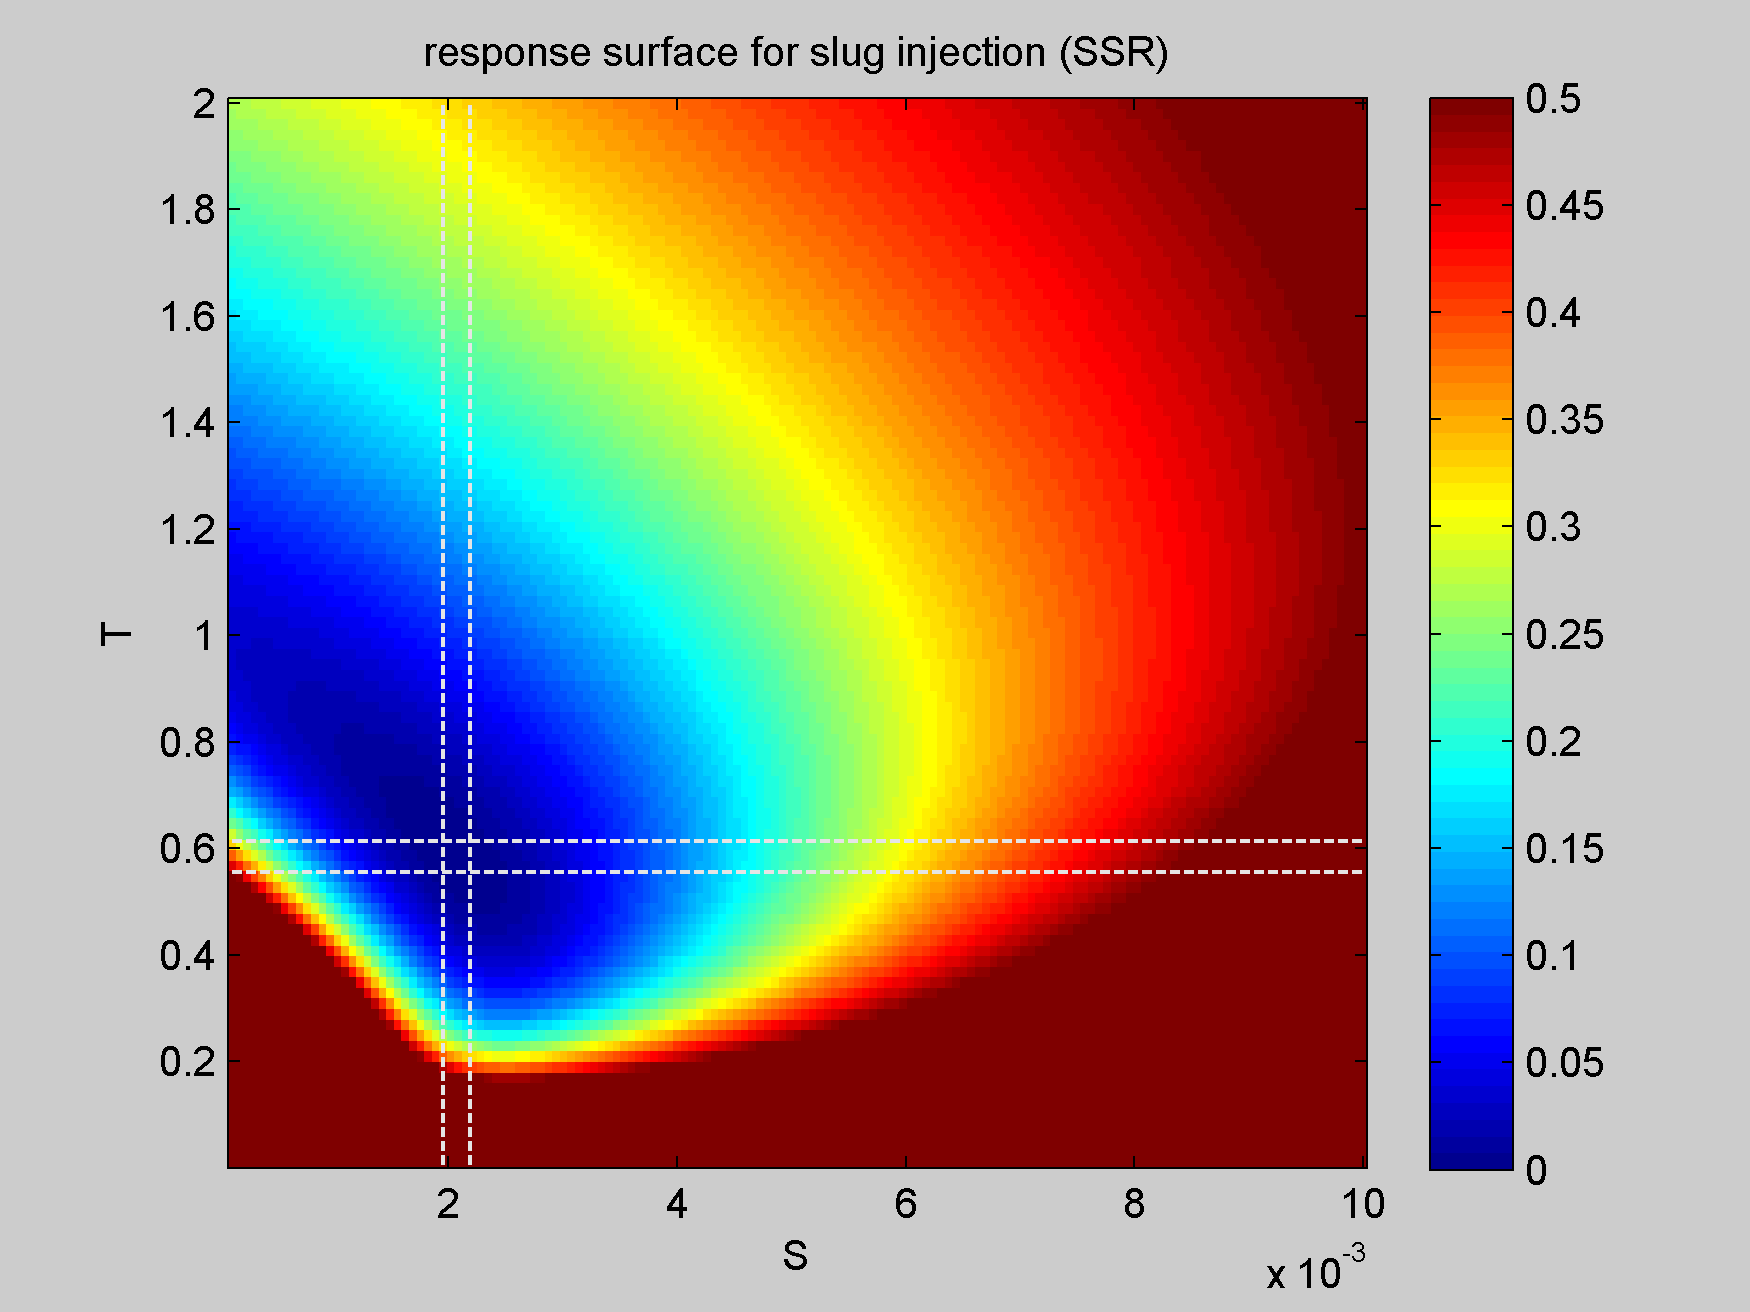
\includegraphics[width=1.0\textwidth]{./eps/converted/respsurf-sluginj}
  \caption{Response surface for the slug injection test. Dotted lines represent
the 95\% confidence interval of the model parameters when the standard deviation
of the head measurement is 0.01~[\textsf{m}].}
  \label{fig:respsurf-sluginj}
\end{figure}


\smallq{The dotted lines in Figure~\ref{fig:respsurf-sluginj} indicate the 95\%
confidence intervals of the model parameters when the standard deviation of the
head measurement is 0.01~[\textsf{m}]. Do you think this is a reasonable
approximation for this nonlinear problem?}


\section{Optimization using local methods}

\subsection{Gauss-Newton and Levenberg-Marquardt}

\smallq{Two algorithms---Gauss-Newton (GN) and Levenberg-Marquardt (LM)--have
been implemented to automatically find the optimal parameters for the slug test.
To run these algorithms for the slug test problem, set your work directory to
`./exercises/local-methods-sluginj'. This directory contains a function that
performs a Gauss-Newton as well as a Levenberg-Marquardt optimization. This
function requires an input argument containing a starting point
(e.g.~\mcode{[0.15,0.4]}). For each method, the function returns an array with a
record of parameter sets and their objective score. You can call the function
from the command line using:

\mcode{[P_GN,P_LM]=Run_Optimization([0.15,0.4]);}
}



\smallq{Have a look at the code and interpret the output.}

\smallq{How quickly does the GN method converge?}

\smallq{How does this compare to the LM method?}

\smallq{Play around with different starting points for the two algorithms. Does
the GN method always converge to the optimum? What about the convergence of the
LM method?}

\smallq{Find a starting point where the GN and LM methods differ and study the
iterations in detail (\mcode{P_GN} and \mcode{P_LM}).}

\smallq{What is the key difference between the iterations of the GN and LM
method?}


\subsection{Multi-start simplex}

HYMOD \citep{boyl-gupt-soro2000} is a simple rainfall-runoff model with 5 model
parameters (see Figure~\ref{fig:hymod}).

\begin{figure}[htbp]
  \centering
    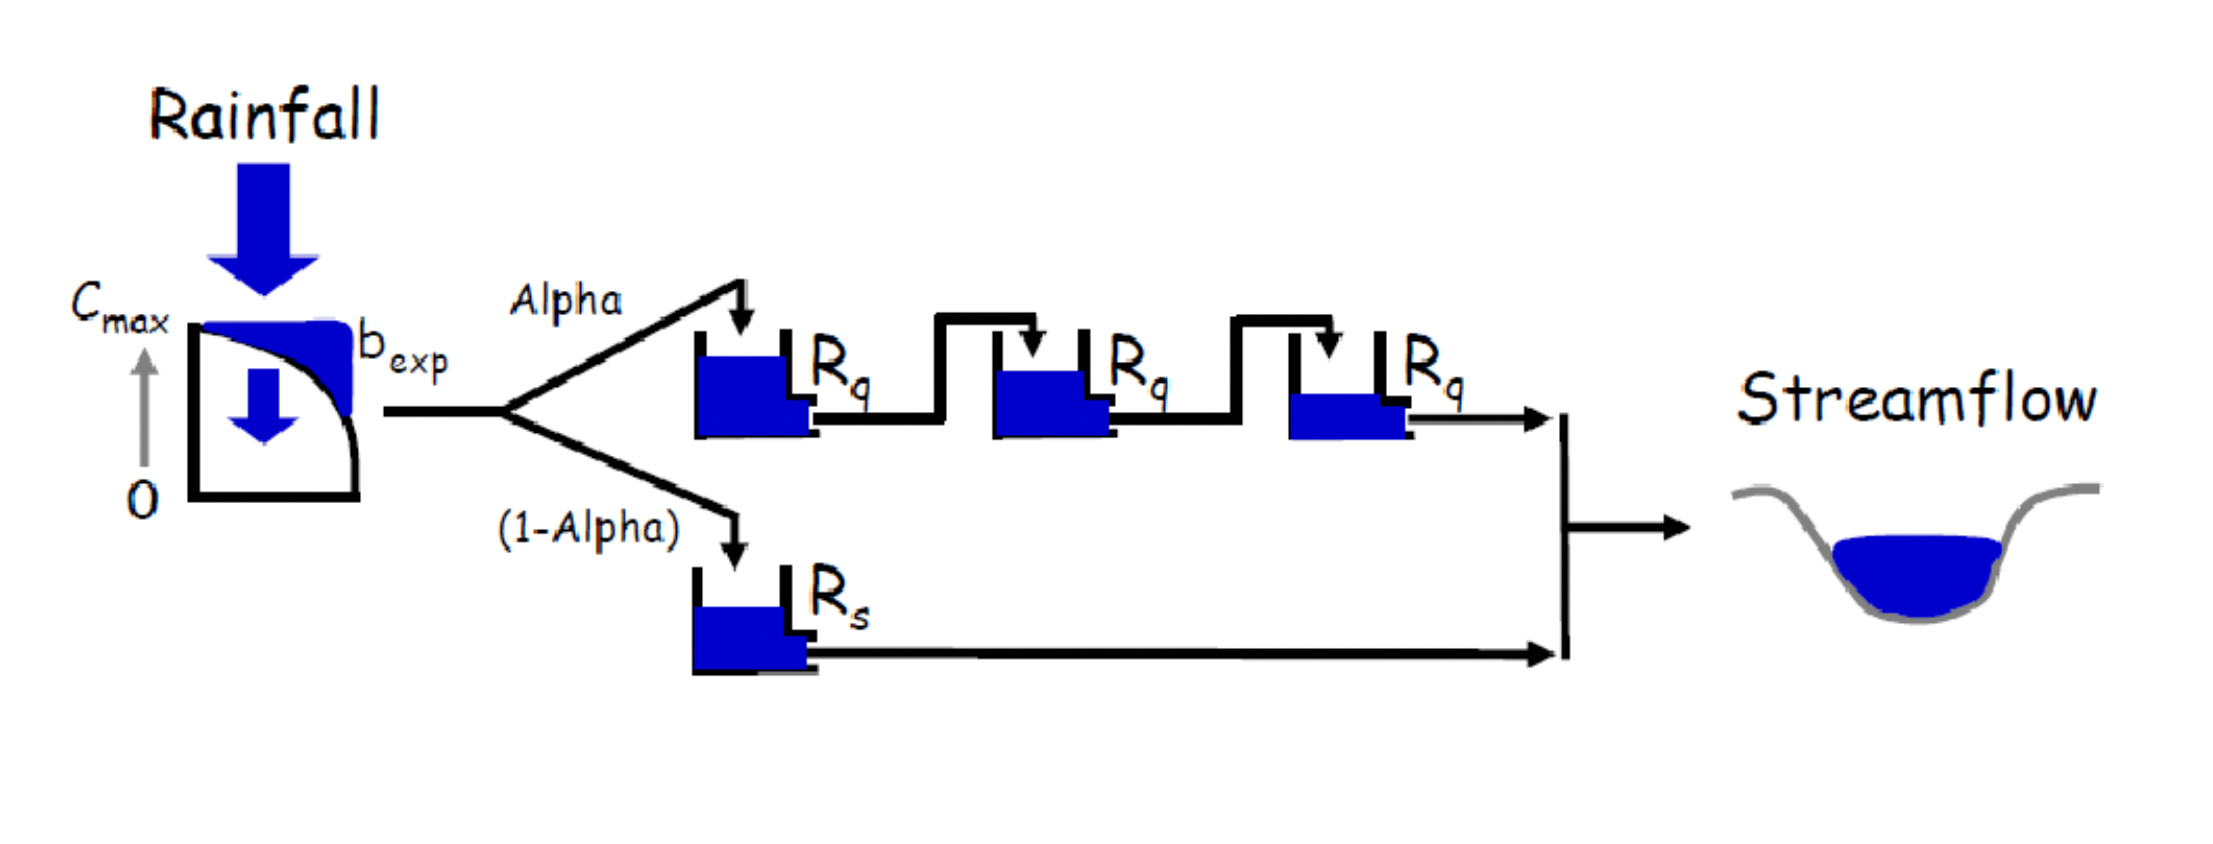
\includegraphics[width=1.0\textwidth]{./eps/converted/hymod}
  \caption{Structure of the HYMOD rainfall-runoff model.}
  \label{fig:hymod}
\end{figure}
\begin{tabular}{ll}
with:&\\
$C_{max}$&Maximum storage of the watershed\\
$b_{exp}$&Spatial variability of soil moisture capacity\\
$Alpha$&Partitioning factor of excess rainfall into slow and quick flow\\
$R_{s}$&Residence time of the slow tank\\
$R_{q}$&Residence time of the quick tanks\\
\end{tabular}

In this section, we will use a multi-start simplex \citep{neld-mead1965} to
optimize the parameters of the HYMOD model. Specifically, we investigate whether
the objective function (SSR) of this model has local minima that may complicate
the use of local optimization methods such as Gauss-Newton, or
Levenberg-Marquardt. To do this, 20 simplex runs are started from randomly
determined starting points, which are iterated until convergence is achieved.

\smallq{First, have a look at the code of `Multistart\_Simplex.m' in
`./exercises/local-methods-hymod/'. As you can see, the code uses the built-in
MATLAB function \mcode{fminsearch}, which is an implementation of the simplex
search algorithm. Run \mcode{Multistart\_Simplex} (it'll run for a few minutes).
Store the output by copy-pasting screenshots into a PowerPoint presentation.}

\smallq{Do all the Simplex runs converge to the same point in the parameter
space?}

\smallq{What does this tell you about the presence of local minima?}

\smallq{For the slug injection test, we visualized the response surface. Can we
make a similar figure here?}

\smallq{When you look at the results of the simulations with optimized
parameters, why do you see just 3 or 4 time series and not 20?}

\smallq{How do you value the results of the various models?}

\smallqo{In the previous exercise, a relatively short data set (3 months) was
used to calibrate HYMOD. Extend the calibration period to 12 months by changing
the values of \mcode{Extra.calPeriod} in  \mbox{`Multistart\_Simplex.m'} and run
the optimization again.}

\smallqo{For this new subset of data, why did the number of local minima
increase or decrease?}

\smallqo{What is the quality of the model runs corresponding to the local
minima?}

\smallqo{If we discard the poor models, can you give an interpretation why these
local minima occurred?}





\section{Global methods: Differential Evolution}


Differential Evolution~\citep{stor-pric1997} is a basic global optimization
algorithm that uses a population of points in the parameter space to find the
global maximum (minimum, if appropriate) of an objective function. Generally
speaking, the population's properties are used to generate more points in those
parts of the parameter space which are most promising with regard to yielding
the global optimum.

\smallq{Use the MATLAB editor to open
`./exercises/differential-evolution/respsurf.m'. This script contains a few
lines of code to help you get started on your algorithm. Run the script to
visualize the response surface for the benchmark function `6' (Shifted
Rosenbrock's  Function) for \mcode{x = [65:0.1:80]} and \mcode{y = [35:0.1:45]}
(Figure~\ref{fig:respsurf-rosenbrock}).}
\begin{figure}[htbp]
  \centering
    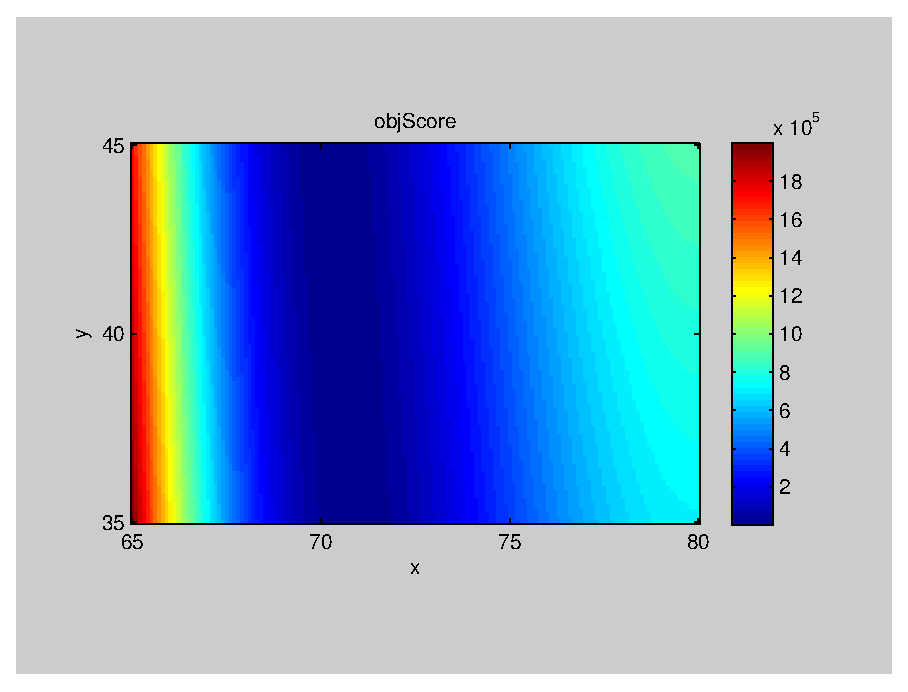
\includegraphics[width=1.0\textwidth]{./eps/converted/respsurf-rosenbrock}
  \caption{Response surface for the shifted Rosenbrock function.}
  \label{fig:respsurf-rosenbrock}
\end{figure}

The \mcode{benchmark_func} function offers not just 1, but 25 functions that can
be visualized in the same way as you already did for the Rosenbrock function.
You can choose different functions by changing the \mcode{funcFlag}. Each
function has its own limits on the parameter space (see
Table~\ref{tab:benchmark-func-data}).

\begin{table}[t]
\centering
\scriptsize
\begin{tabular}{lp{9cm}l}
\mcode{funcFlag}&\textbf{description}&\textbf{limits}\\
\multicolumn{3}{l}{Unimodal Functions (5):}\\
1  &Shifted Sphere Function                                                              & [-100,100]\\
2  &Shifted Schwefel's Problem 1.2                                                       & [-100,100]\\
3  &Shifted Rotated High Conditioned Elliptic Function                                   & [-100,100]\\
4  &Shifted Schwefel's Problem 1.2 with Noise in Fitness                                 & [-100,100]\\
5  &Schwefel's  Problem 2.6 with Global Optimum on Bounds                                & [-100,100]\\
\multicolumn{3}{l}{Multimodal Functions (20):}\\
\multicolumn{3}{l}{Basic Functions (7):}\\
6  &Shifted Rosenbrock's Function                                                        & [-100,100]\\
7  &Shifted Rotated Griewank's Function without Bounds                                   & [0,600]\\
8  &Shifted Rotated Ackley's Function with Global Optimum on Bounds                      & [-32,32]\\
9  &Shifted Rastrigin's Function                                                         & [-5,5]\\
10  &Shifted Rotated Rastrigin's  Function                               & [-5,5]\\
11  &Shifted Rotated Weierstrass Function                                & [-0.5,0.5]\\
12  &Schwefel's  Problem 2.13                                            & [-100,100]\\
\multicolumn{3}{l}{Expanded Functions (2):}\\
13  &Expanded Extended Griewank's  plus Rosenbrock's  Function (F8F2)                    & [-3,1]\\
14  &Expanded Rotated Extended Scaffe's  (F6)                                & [-100,100]\\
\multicolumn{3}{l}{Hybrid Composition Functions (11):}\\
15  &Hybrid Composition Function 1                                       & [-5,5]\\
16  &Rotated Hybrid Composition Function 1                               & [-5,5]\\
17  &Rotated Hybrid Composition Function 1 with Noise in Fitness                     & [-5,5]\\
18  &Rotated Hybrid Composition Function 2                               & [-5,5]\\
19  &Rotated Hybrid Composition Function 2 with a Narrow Basin for the Global Optimum    & [-5,5]\\
20  &Rotated Hybrid Composition Function 2 with the Global Optimum on the Bounds         & [-5,5]\\
21  &Rotated Hybrid Composition Function 3                           & [-5,5]\\
22  &Rotated Hybrid Composition Function 3 with High Condition Number Matrix         & [-5,5]\\
23  &Non-Continuous Rotated Hybrid Composition Function 3                        & [-5,5]\\
24  &Rotated Hybrid Composition Function 4                               & [-5,5]\\
25  &Rotated Hybrid Composition Function 4 without Bounds                            & [-2,5]\\
\end{tabular}
\caption{}
\label{tab:benchmark-func-data}
\end{table}

\smallq{Experiment with different functions to get some idea of what their
response surfaces look like.}

%\hspace*{0.01mm}
%\vfill
%\hspace*{0.01mm}


\needspace{8\baselineskip}
In the next few exercises, you will write your differential evolution algorithm.
We will take you through the following basic steps (see also
\textsf{Fig.~\ref{fig:diff-evo-principle}} and \textsf{Code
Snippets~\ref{list:generating-uniform-random-sample}} and
\textsf{\ref{list:generating-proposals}}):
\begin{enumerate}
\item{generate the initial sample;}
\item{assign the initial sample to a new array \mcode{parents};}
\item{for each sample in \mcode{parents}, calculate the corresponding objective
score;}
\item{use \mcode{parents} to calculate new \mcode{proposals};}
\item{for each sample in \mcode{proposals}, calculate the corresponding objective
score;}
\item{accept either a sample from \mcode{proposals} or the corresponding sample
from \mcode{parents} as the child, thus making an array \mcode{children} of the
same size as \mcode{parents};}
\item{assign \mcode{children} to \mcode{parents} for the next generation, and go
back to step 4.}
\end{enumerate}

\begin{figure}[htbp]
  \centering
    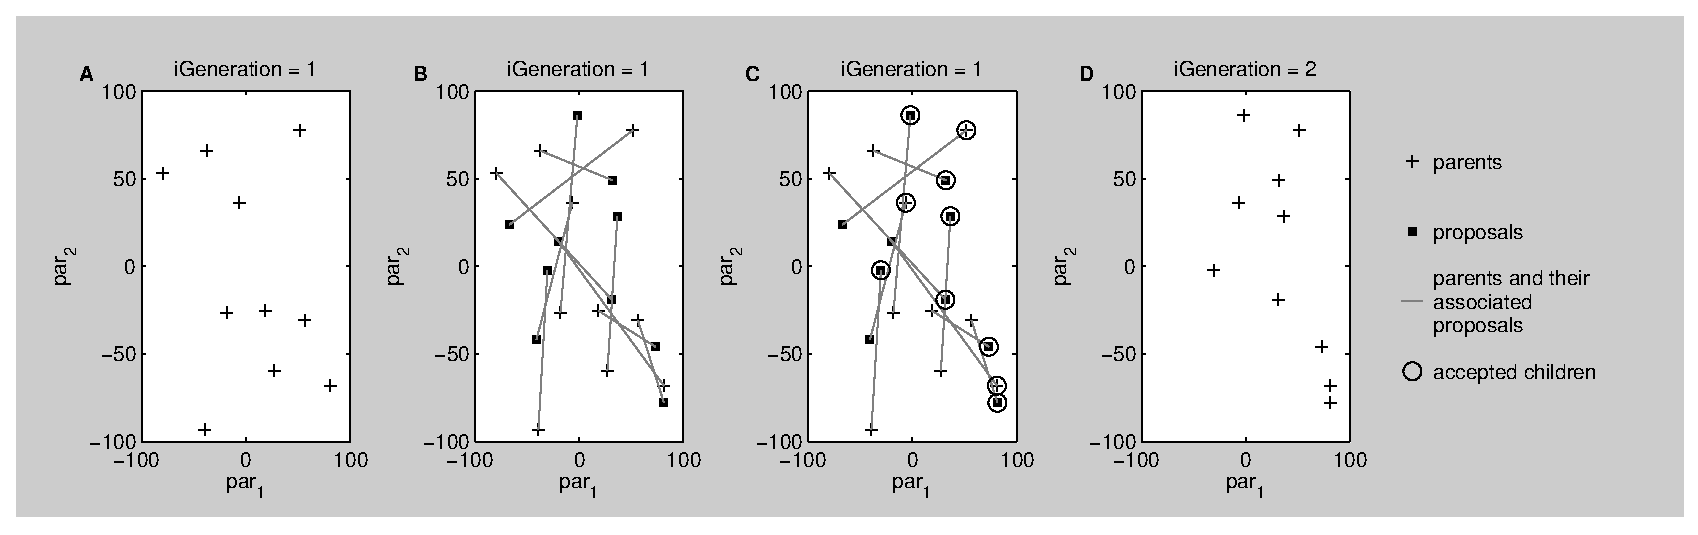
\includegraphics[width=1.0\textwidth]{./eps/converted/diff-evo-principle}
  \caption{Differential evolution in a nutshell, using a population of
  \texttt{nPop = 10} to avoid cluttering the figures. \textbf{A}:~Generation of
  the initial sample. \textbf{B}:~Generation of proposal points.
  \textbf{C}:~Accepting either a sample from \texttt{parents} or from 
  \texttt{proposals} as a row in \texttt{children}. \textbf{D}:~The 
  \texttt{children} from one generation are the \texttt{parents} for the
  next generation.}
  \label{fig:diff-evo-principle}
\end{figure}

\lstinputlisting[float=ht,caption={Generating samples drawn from a uniform
distribution spanning the parameter
space.},label=list:generating-uniform-random-sample]{./m/snippet-diff-evo-generating-uniform-random-sample.m}

\lstinputlisting[float=ht,caption={Generating proposal points given a parent
population.},label=list:generating-proposals]{./m/snippet-diff-evo-generating-proposal-points.m}


\smallq{As a first step, save your \mcode{respsurf} script under a new name
`runDiffEvo.m'.}

\smallq{Extend `runDiffEvo.m' by creating an array \mcode{parents}, which has
\mcode{nPop=50} rows, each of which represents a uniform random sample from the
parameter space (see also \textsf{Code
Snippet~\ref{list:generating-uniform-random-sample}}). \mcode{parents} has
\mcode{nDims+1} columns, i.e. the number of dimensions for which you want to
solve \mcode{benchmark_func} plus one column to store the objective score. Refer
to Table~\ref{tab:benchmark-func-data} for the parameter space limits. For now,
stick with \mcode{nDims=2} and \mcode{funcFlag=6}, but you can change that
later.}

\smallq{Calculate the last column of \mcode{parents} by running the objective
function for each row.}

\smallq{Generate the \mcode{proposals} array (same size as \mcode{parents}). To
do this, select the first sample from \mcode{parents}, as well as three other
samples (\mcode{r1}, \mcode{r2}, \mcode{r3}), chosen at random from
\mcode{parents} (MATLAB's built-in function \mcode{randperm} can be useful for
this; see \textsf{Code Snippet~\ref{list:generating-proposals}}). The proposal
is calculated as the position of the parent + F*\mcode{dist1} + K*\mcode{dist2},
in which  \mcode{dist1} is the distance between the parent and \mcode{r1},
\mcode{dist2} is the distance between \mcode{r2} and \mcode{r3}, and F and K are
settings that are part of the Differential Evolution algorithm. In the
literature, F=0.6 and K=0.4 are common. Repeat for all samples in
\mcode{parents}.}

\smallq{For each member in \mcode{proposals}, calculate the objective score.}

\smallq{Determine whether to choose the $i^{th}$ sample of \mcode{parents} or
the $i^{th}$ sample of \mcode{proposals}, depending on which one has a better
objective score. Assign to the $i^{th}$ row in a new array \mcode{children}.}

\smallq{Assign \mcode{children} to \mcode{parents} for the next generation.}

\smallq{Wrap most of the above steps in a \mcode{for} loop, such that your
script will repeatedly generate new (and hopefully better) children for 250
generations.}

\smallq{It's a little bit difficult to see if your script is doing what it is
supposed to be doing, so you need to do some visualization. Copy and paste from
`vis-helper.txt' to create a figure similar to Figure~\ref{fig:diffevo-result}.}

\begin{figure}[htbp]
  \centering
    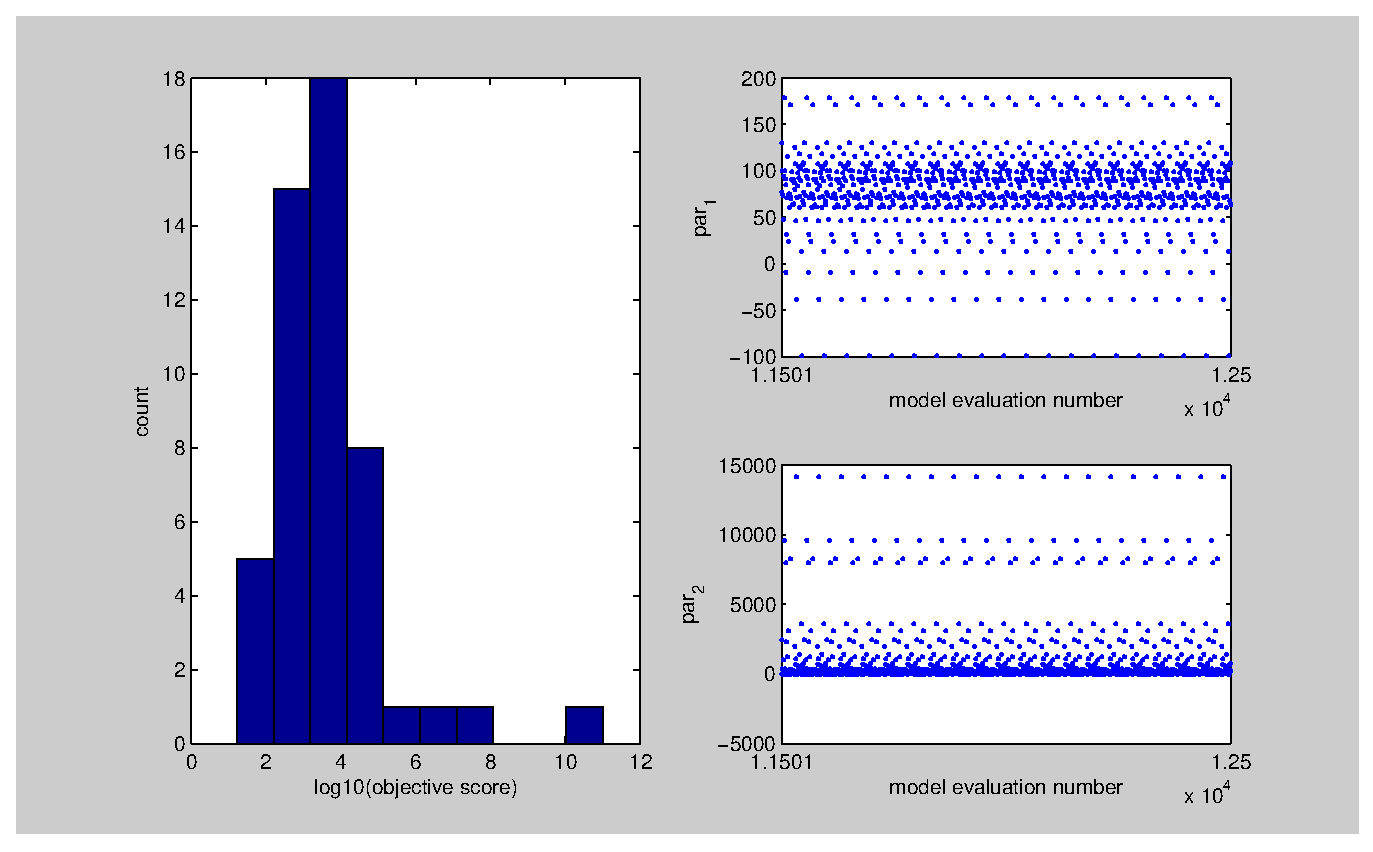
\includegraphics[width=1.0\textwidth]{./eps/converted/diffevo-result}
  \caption{Visualization results for the Shifted Rosenbrock function after 250
  generations of 50 samples each, optimized using the Differential Evolution
  algorithm.}
  \label{fig:diffevo-result}
\end{figure}



\smallq{During the optimization, you may notice that there are some points that
are really persistent, even though they are well away from the global optimum.
Explain why these points are so persistent.}

\smallq{The histogram in Figure~\ref{fig:diffevo-result} is bimodal. How does
that relate to the answer to the previous question?}





%\chapter{Working with DREAM}
\thispagestyle{fancy}
\label{ch:Working-with-DREAM}


\hrule
\begin{itemize}
\footnotesize
\item[]{Aims:}
\begin{enumerate}
\item{to understand the functionality of DREAM;}
\item{to understand the basics of the implementation of DREAM;}
\item{to experience the process of parameter evolution;}
\item{to understand the implementation of a (linear) model in DREAM;}
\item{to experience the changes that need to be made when a new model is implemented in DREAM.}
\end{enumerate}
\end{itemize}
\hrule
\vspace{1em}

Before we can start optimizing the parameters for any model, we need to set up the DREAM algorithm \citep{vrug-terb-diks-robi-hyma-higd2009}. An efficient way of doing this is by creating a new m-file, that consists of 5 parts, which are used to:
\begin{enumerate}
\item{clean up any old variables, figures etc. and add the DREAM folder to the MATLAB search path. This way, you can access the functions that make up the DREAM algorithm, even though they do not reside in the current working folder;}
\item{load or create any data that you will need during the optimization. This includes the observations but also the model constants, intial conditions, etc.;}
\item{specify the settings with which to run the DREAM algorithm. The most important variables that need to be initialized in this part are 4 structure arrays: \mcode{MCMCPar, ParRange, Measurement, Extra};}
\item{call the DREAM algorithm;}
\item{visualize, analyze, and post-process the outcome of the optimization.}
\end{enumerate}


We have included an example of how DREAM can be used to calibrate the parameters of a linear model. The example is located at `./exercises/dream-linear-model/'. 

\smallq{Use the MATLAB editor to open `dreamWithLinearModel.m'.}

In the DREAM settings part, the user typically adjusts the number of parameters (\mcode{MCMCPar.n}), the maximum number of model evaluations (\mcode{MCMCPar.ndraw}), the limits of the parameter space (\mcode{ParRange}), the measurements to be used in the objective function (\mcode{Measurement}), and of course the name of the function whose parameters are optimized (\mcode{ModelName}). Any additional arrays that the model needs to run---initial conditions, boundary conditions etc.--can be included as fields in the structure array \mcode{Extra}. 


On the model side, DREAM has a few small requirements also; DREAM expects models to be formulated as a function with two input arguments, the first being a parameter vector of length \mcode{MCMCPar.n} and the second a structure array with additional data (initial conditions, boundary conditions, and anything else you need inside the function).

\smallq{Open `linearmodel.m' in the MATLAB editor to see how this works.}

Note that DREAM compares the model output directly to the measurements stored in \mcode{Measurement.MeasData}, so they should have the same dimensions for this to work. Also, for the comparison to make sense at all, you need to make sure that the values in the model output and in the measurement correspond to the same point in time (or space). Models that use a variable time step can be especially tricky in this respect.

\smallq{If you didn't already do this, run `dreamWithLinearModel'.}

During the optimization, you will see some figures being created automatically. Depending on which figures you want to see, you can set the \mcode{visualize*} variables in `visDream.m' as you like. Furthermore, you can adjust the interval at which figures are plotted by setting \mcode{visInterval}, further down in `visDream.m'.

\smallq{Set your work directory to `./exercises/dream-quadratic-model'. The model m-file in this directory is `quadraticmodel.m'. Write a main script similar to `dreamWithLinearModel.m', with which the parameters of the quadratic model are optimized. Copy and paste from the linear model example as appropriate.}


\smallq{After the optimization finishes, it's often desirable to save the variables and figures to harddisk, for example by:
\lstinputlisting[numbers=none,nolol,label={lst:save-print}]{./../m/save-print.m}
This is especially useful for cases in which the model takes a bit of time to run. 
}% smallq

%\chapter{Objectives and information in data}
\thispagestyle{fancy}
\label{ch:objectives-and-information-in-data}



\hrule
\begin{itemize}
\footnotesize
\item[]{Aims:}
\begin{enumerate}
\item{to be aware of the added value of carefully interpreting the results of the parameter evolution;}
\item{to understand the effect of noise in the measurements;}
\item{to understand the effect of the distribution of observations in relation to the model's local sensitivity (or system behavior);}
\item{to experience the added value of data transformations for parameter identification;}
\item{to understand the consequences of model structural errors for the parameter optimization process and result;}
\item{to experience the opportunities of multi-objective optimization.}
\end{enumerate}
\end{itemize}
\hrule
\vspace{1em}




%\section{Guided discussion ``Objective functions''}
%
%\smallq{Answer the following questions individually (allotted time: 15 minutes)
%\begin{itemize}
%\item{What is the aim of your research (in general, modeling is not an aim but it may be a means to reach your aim)?}
%\item{Why do you use modeling in your research?}
%\item{What could you learn from inverse modeling in your research?}
%\item{Describe the model results that you could confront with measurements and describe these measurements (diagnostic variables)}
%\end{itemize}
%}%smallq
%
%
%\smallq{Now exchange information within the group (allotted time: 30 minutes). Each member of the group explains his/her research to the rest of the group in 5 minutes. After a short introduction, also pay attention to the issues above. Other group members ask for clarification if needed.}
%
%\smallq{Choose one of the studies for further explanation and evaluation (allotted time: 5 minutes). The best choice is:
%\begin{itemize}
%\item{concrete, both in model concept and data;}
%\item{not already used in a inverse modeling context;}
%\item{not too much the same as the examples that we have already discussed in the lectures and exercises.}
%\end{itemize}
%}%smallq
%
%
%\smallq{For the case that your group chose,
%\begin{itemize}
%\item{List the system properties/parameters in the model;}
%\item{Which of these can be measured? How?}
%\item{Can you measure these at the same scale/support/extent as used in the model?}
%\item{Which ones would you use in your inverse modeling procedure? Why?}
%\item{How would you formulate your objective? Why?}
%\item{What conclusions do you hope to draw from the inverse modeling activity?}
%\item{How does this relate to your research aims, as you have formulated?}
%\end{itemize}
%}%smallq
%
%\section{Model complexity, measurement error, and what to measure}

Often people perform a model calibration, then they present the final model result, and then\ldots they are done. But in fact the most interesting part of inverse modeling is the interpretation of both the results of the evolution of the parameter search and of the simulation results. In this chapter, we will investigate the relation between model complexity, measurement error, and the type of observations.

\section{Case: cubic model}

\smallq{Use the MATLAB editor to open `dreamWithCubicmodel.m' located in `./exercise/dream-cubicmodel/'. After briefly studying the program, press F5 to run it as provided with 14 data points (variables \mcode{xObs} and \mcode{yObsNoisy}). Don't forget to save the results (check the code snippet on page~\pageref{lst:save-print} or copy and paste in a PowerPoint presentation).}

\smallq{To identify the parameters of a 4-parameter model, 14 data points aren't very many. How do you think the results will change if you increase the number of data points? Check your hypothesis by setting \mcode{xObsStep} to 0.2.}

\smallq{Not only the number of the data points is important, but also the distribution. Argue what would be the result if you wouldn't have had the data points below x=3 (keep \mcode{xObsStep} at 0.2). Explain which parameters you expect to be identified most accurately? Then check whether your hypothesis was correct.}

\smallq{If you could do one more measurement between x=-1 and x=7, where would you place it? Explain why.}

\smallq{What if you would have only the observations below x=3 (keep \mcode{xObsStep} at 0.2)? Again, explain which parameters you expect to be identified most precisely and then check whether your hypothesis was correct.}

\smallqo{If you would increase the magnitude of the error term (\mcode{gaussTerm}), how will that affect the results? Check your hypothesis by making the appropriate changes to the script.}

\section{Case: rainfall interception}

In this part, we will interpret the relation between data, model and selected parameters using a simplified version of an existing rainfall interception model \citep{bout-scha-aert-verm1996}. This version simulates canopy water storage using one layer only. As with any model, it is important that you understand both the concept of the model---including equations, parameters and boundary conditions---as well as the measurements used in the inverse modeling; if you don't, it is impossible to interpret the results.

Conceptually, the interception model is a very simple water balance of the canopy. Water storage in the canopy (S) changes with time $t$, as a result of precipitation (P), interception (I), drainage (D) and evaporation (E); see Figure~\ref{fig:interception-model-flows} and Equation~\ref{eq:interception-model}.
\begin{equation}
\label{eq:interception-model}
\frac{\Delta S}{\Delta t} = I-D-E
\end{equation}
\begin{tabular}{lll}
with:&&\\
$S$&canopy water storage&\textsf{mm}\\
$t$&time&\textsf{day}\\
$I$&interception rate&\textsf{mm$\cdot{}$day$^{-1}$}\\
$D$&canopy drainage rate&\textsf{mm$\cdot{}$day$^{-1}$}\\
$E$&canopy evaporation rate&\textsf{mm$\cdot{}$day$^{-1}$}\\
\end{tabular}

\begin{figure}[htbp]
  \centering
    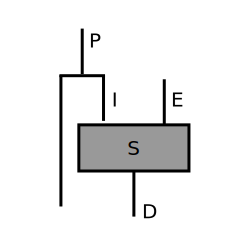
\includegraphics[width=0.3\textwidth]{./eps/converted/interceptionmodel-flows}
  \caption{Definition of flows for the interception model.}
  \label{fig:interception-model-flows}
\end{figure}

\needspace{5\baselineskip}Precipitation and potential evaporation ($E_0$) are the measured boundary conditions. The other fluxes are calculated as:
\begin{equation}
I=a\cdot{}P
\end{equation}
\begin{equation}
D =
\begin{cases}
b\cdot{}(S-c), & \text{if }S>c\\
0, & \text{if }S\leq{}c\\
\end{cases}
\end{equation}
\begin{equation}
E = d\cdot{}E_0\cdot{}\frac{S}{c}
\end{equation}
\begin{tabular}{lll}
{\bf parameter}&{\bf description}&{\bf units}\\
$a$&interception efficiency (canopy cover fraction)&\textsf{-}\\
$b$&canopy drainage efficiency&\textsf{day$^{-1}$}\\
$c$&canopy water storage capacity&\textsf{mm}\\
$d$&evaporation efficiency&\textsf{-}\\
\end{tabular}



Before optimizing the model parameters $a$, $b$, $c$ and $d$, you need to get a better understanding of the meaning of each parameter, and its effect on the model prediction. With this knowledge you will be able to choose a more meaningful minimum and maximum parameter space and your optimization will converge faster.

\smallq{Use the MATLAB editor to open `mancal\_interceptionmodel' located in `./exercises/manual-calibration-interception-model/'. After pressing F5 to run the script, a graphical user interface (GUI) will appear. If you run the model with the input values $a$ = 0.6, $b$ = 200, $c$ = 2.5 and $d$ = 0.83, you will get a plot similar to those in  Figure~\ref{fig:interceptionmodel-mancal-gui}. Explain the output of this simulation:

\begin{itemize}
\item{why does the storage increase at $t$ = 0.75?}
\item{why does it reach a constant level?}
\item{why is this level 2.6?}
\item{why does this level change at $t$ = 1.0?}
\item{why does this level become 2.5?}
\item{why does the storage decrease at $t$ = 1.25?}
\item{explain the shape of the storage curve after $t$ = 1.25.}
\item{draw the canopy evaporation rate in Figure~\ref{fig:interceptionmodel-mancal-gui}.}
\end{itemize}
}% smallq

\begin{sidewaysfigure}
%\begin{figure}[htbp]
  \centering
    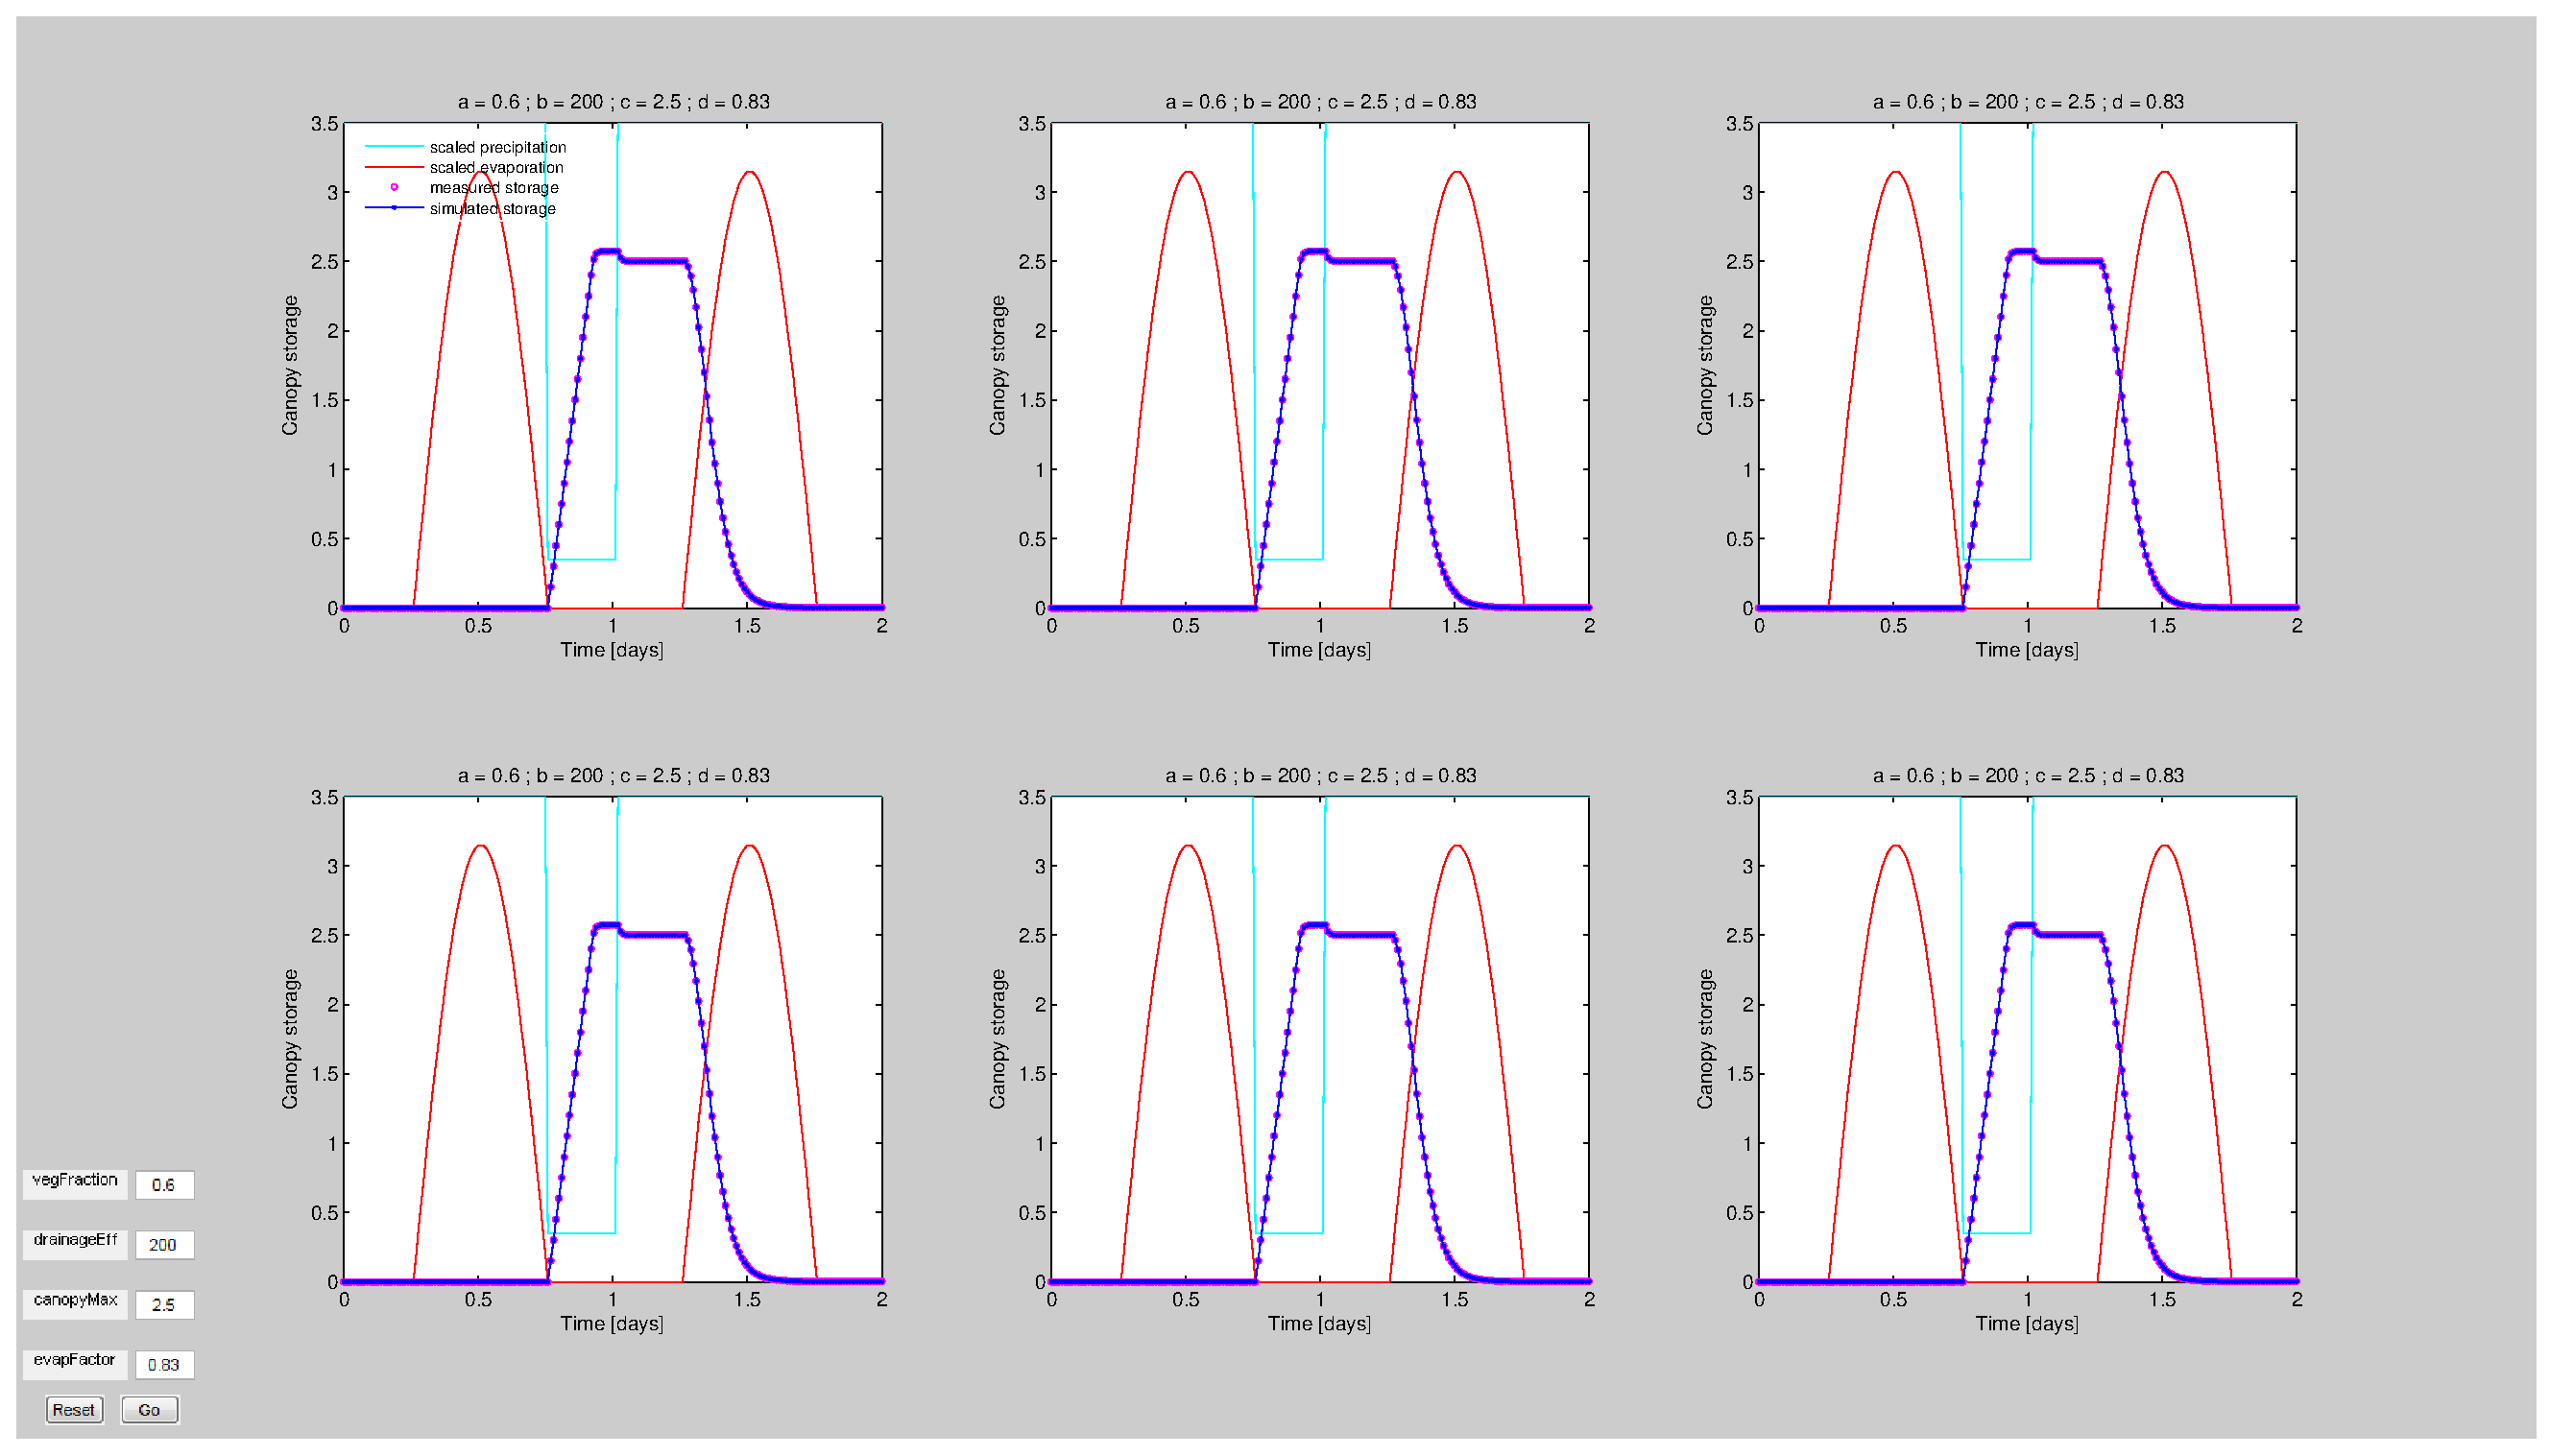
\includegraphics[width=1.0\textheight]{./eps/converted/interceptionmodel-mancal-gui}
  \caption{Graphical user interface showing the model prediction for $a$ = 0.6, $b$ = 200, $c$ = 2.5 and $d$ = 0.83, based on simplified boundary conditions.}
  \label{fig:interceptionmodel-mancal-gui}
%\end{figure}
\end{sidewaysfigure}

\smallq{Next we will alter the parameter values only one at a time (!) and predict how the change affects the model result. So, choose a parameter, then first draw your prediction in one of the subplots of Figure~\ref{fig:interceptionmodel-mancal-gui}. Only after you've drawn your prediction, change the parameter value in the GUI. Press the `Go' button to run the interception model with the changed parameter. Try to explain why your prediction diverges from the model result. This is a useful procedure to better understand the behavior of a system.}

\smallq{Summarize the knowledge you gained about each parameter's effect on the model result.}

\subsection{Distribution of information within the data}

Having done the manual calibration, you are ready to interpret the results of the interception model with boundary conditions that are more realistic. In the next few exercises, we will perform several DREAM calibrations of the interception model using  different data sets.

As a first step, it is always wise to first check your inverse modeling design with so-called `artificial measurements'. Artificial measurements are generated by running the model with a known parameter set. Subsequent calibration of the model to the artificial measurements should yield this same parameter set again.

\smallq{Use the MATLAB editor to open `dreamWithInterc.m' located in `./exercises/dream-interception-model/'. By default this script uses the simplified boundary condition that we used in the manual calibration. Run the main script to check if the true parameters are found.}

\smallq{Now adapt your script to let it use the more realistic boundary conditions, by uncommenting the appropriate parts in the script. Experiment with different boundary conditions. Can you explain the differences between the various data sets? And what is the difference between the realistic boundary conditions on the one hand and the ideal case on the other?}

It is often interesting to calibrate your model parameters based on a subset of the data. This way, you can get some idea of the type of information that is needed to identify each model parameter with precision and accuracy. The generic way to have DREAM use subsets, is by adding a field to \mcode{Extra} that contains the observation times that you want to use as part of your objective function:
\lstinputlisting[numbers=none,nolol,label={lst:subsetting-t-less-than-one}]{./../m/subsetting-t-less-than-one.m}
\needspace{3\baselineskip}Inside \mcode{interceptionmodel}, you can use the time information to only export simulated storage values at the times specified in \mcode{tObj}:
\lstinputlisting[numbers=none,nolol,label={lst:subsetting-modelside}]{./../m/subsetting-modelside.m}
\mcode{output} can subsequently be returned as the function's output argument, after which DREAM will compare it to the contents of \mcode{Measurement.MeasData}.


\needspace{15\baselineskip}After the optimization finishes, the script probably throws an error in the visualization part. This is because the simulated time series of storage now has less elements than \mcode{bounds(:,1)}. You can avoid this by re-defining \mcode{Extra.tObj} just before re-running the last 1000 parameter sets:
\lstinputlisting[numbers=none,nolol,label={lst:subsetting-redefine-extra}]{./../m/interceptionmodel-subsets-redefine-extra.tobj.m}

\smallq{Adapt your script to let it use only the observations for which $t<1$ (simplified boundary conditions). Make sure that the storage values returned by \mcode{interceptionmodel} refer to the times at which storage was observed. What do you expect with regard to the identifiability of the parameters? Store the results to be able to refer back to them later, for instance by copying and pasting into a PowerPoint presentation.}

\smallq{\needspace{5\baselineskip}In the previous exercises, we have calibrated to a time-based subset of the observations. However, you can also make a subset based on certain characteristics of the data. For instance, make a subset based on $S>2.2$~\textsf{mm} (use the `211' data), calibrate the interception model and explain the results. Remember, you can add fields to \mcode{Extra} with information you need inside your model's workspace. For instance, you could do:
\lstinputlisting[numbers=none,nolol,label={lst:subsetting}]{./../m/subsetting.m}
}

\smallq{If you didn't already do this, adapt the script such that the simulated canopy storage dynamics are visualized starting from t=211.41 through t=212.65. Let your visualization differentiate between observations that are part of the objective set and those that aren't. You should get a figure more or less like Figure~\ref{fig:interception-model-subsets}.
\begin{figure}[htbp]
  \centering
    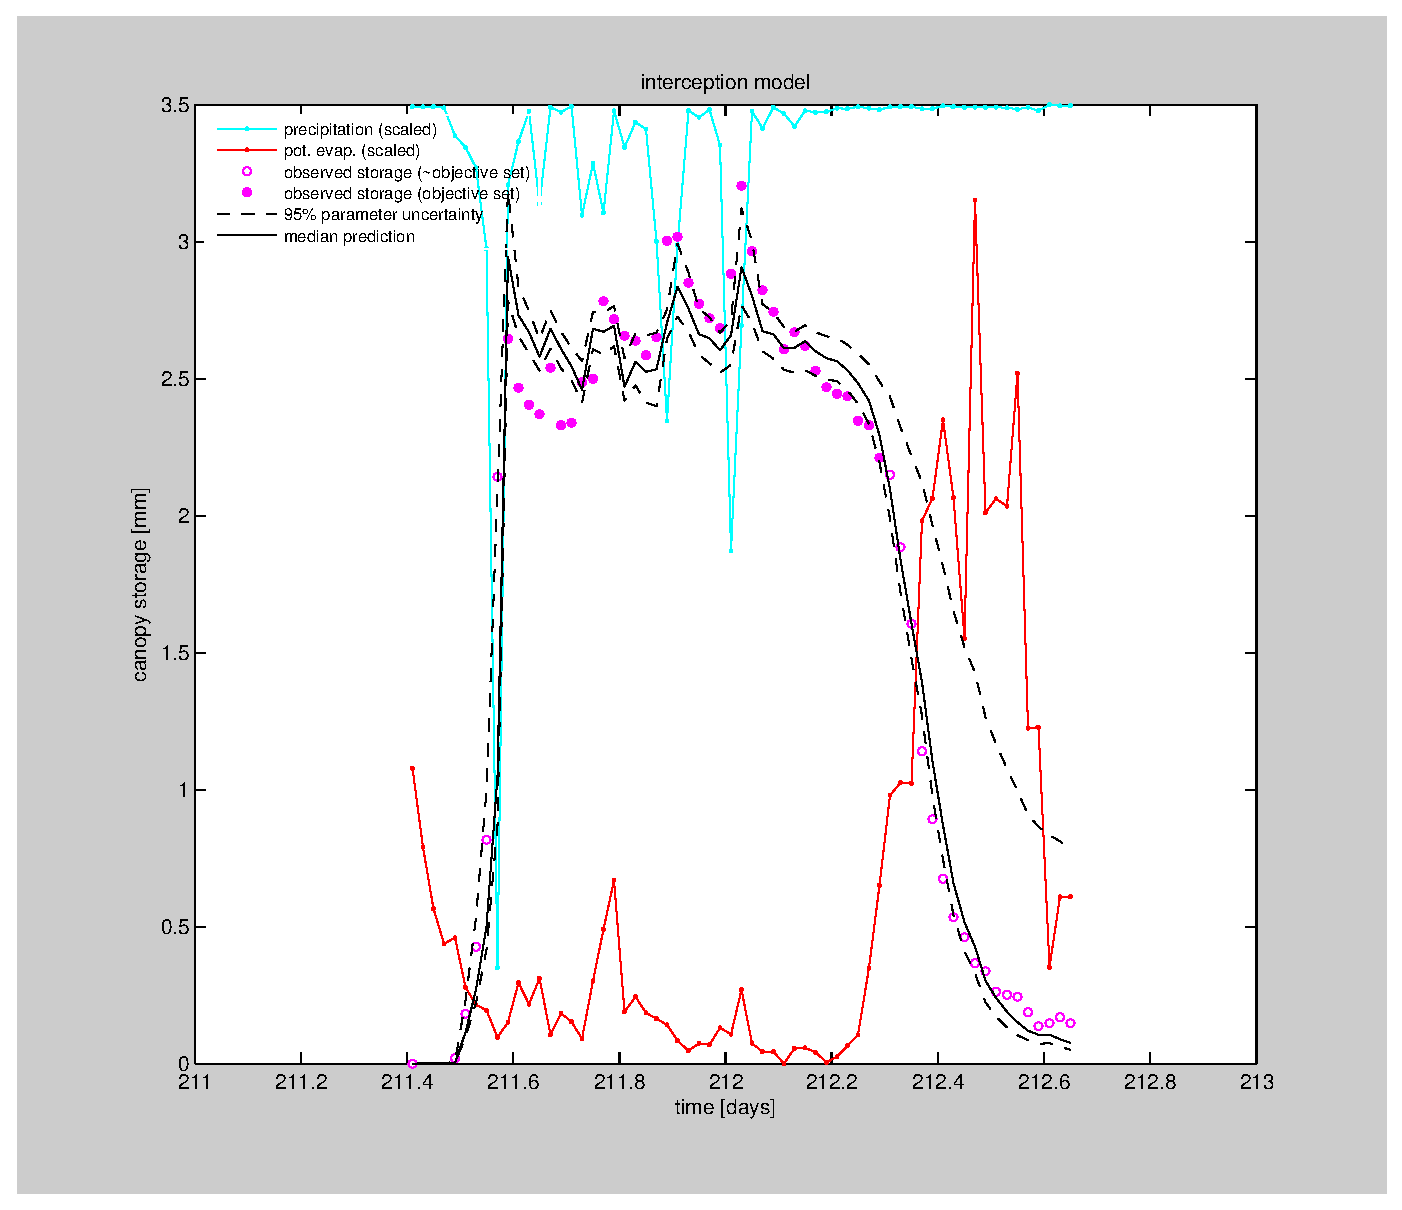
\includegraphics[width=1.0\textwidth]{./eps/converted/interceptionmodel-subset}
  \caption{Example of the interception model with objective based on high-storage values only.}
  \label{fig:interception-model-subsets}
\end{figure}
}% smallq

\smallq{Describe the characteristics of a minimal data set with which the parameters of the interception model can still be identified. Does the measurement accuracy affect the minimal set?}


\subsection{Data transformations}

In this part, we will experiment with using different kinds of transformations. For instance, squaring the observed data ($Y^2$) emphasizes the high values, whereas $\sqrt{Y}$ and Box-Cox transforms ($\frac{Y^\lambda-1}{\lambda}, \lambda=0.3$) give more weight to lower (non-negative) values. Also, Box-Cox transformations are often used when the error is known to be heteroscedastic (i.e.~when the magnitude of the error is dependent on measurement value). $log(Y)$ and $log_{10}(Y)$ should be avoided if Y-values of 0 can occur.

\smallq{Use the MATLAB editor to open `dreamWithHymodBoxCox.m' located in `./exercises/dream-hymod-box-cox'. Despite its name, the script does not perform a Box-Cox transform yet, but we'll get to that in a minute. First run the script as provided and interpret the results.}

\smallq{What change in model performance or identifiability of parameters would you expect if you apply the Box-Cox transform? Before running the script, we need to make some small changes first. Of course, you need to transform the observations as well as the model output. In order to  visualize the optimization results, we need to adapt the model such that it can output either the untransformed simulated storage or the transformed simulated storage, depending on a flag \mcode{Extra.argOutIsTransformed} which can be \mcode{true} or \mcode{false}. For instance:
\lstinputlisting[numbers=none,nolol,label={lst:argOutIsTransformed-modelside}]{./../m/argOutIsTransformed-modelside.m}
This is an easy way to use transformed data for the optimization, and untransformed data for the subsequent visualization. Make the appropriate changes in the program and check the answer you gave earlier.}

Another interesting transform is to use the derivative of the observations. This can be particularly helpful with determining rates with respect to time.

\smallqo{What result do you expect if you apply the derivative transformation in case of the cubic model?}

\smallq{Use the MATLAB editor to open `dreamWithIntercDerivative.m' located at `./exercises/dream-interceptionmodel-derivative/'. As you can see, the objective function operates on the derivative of storage. How do you think the prediction will be different from the earlier results? Check your answer by running the script.}



\section{Case: Easter Island population dynamics}


In the past few exercises we have seen that successful parameter identification depends on what we call ``the information content of data''. It depends on:
\begin{enumerate}
\item{the signal/noise ratio (the higher the ratio, the faster the convergence of the search procedure);}
\item{the sensitivity of the model for the parameters;}
\item{the distribution of the measurements in relation to this sensitivity.}
\end{enumerate}

Keep in mind that a model is never perfect and that deviations between model output and observations is not by definition a Gaussian distribution. If the model structure causes systematic errors, the inverse modeling procedure as used until now will lead to a best fit while tuning the parameters. In this case the optimal parameter values will compensate for the model structure error. In such a case parameter identification produces the ``wrong'' (but optimal) parameter values and convergence will also become slower.

To explore this effect in more detail, we will test a model of human population and resources (trees/biomass) of Easter Island in the period 0-2000 AD. The model is based on \citeauthor*{bran-tayl1998}~(\citeyear{bran-tayl1998}). The governing equations and probable parameter values are as follows.

\needspace{15\baselineskip}

Rate of change of population:
\begin{equation}
\frac{dP}{dt} = (b+cr\cdot{}\frac{C}{P})\cdot{}P-(d-cr\cdot{}\frac{C}{P})\cdot{P}
\end{equation}
Rate of change of resources:
\begin{equation}
\frac{dR}{dt} = g\cdot{}(1-\frac{R}{Cc})\cdot{}R-C
\end{equation}
Consumption rate:
\begin{equation}
C = p\cdot{}P\cdot{}R
\end{equation}

\begin{tabular}{llll}
with:&&&\\
&\textbf{variable name as used}&\textbf{description}&\textbf{probable value}\\
&\textbf{in the model}&&\\
$P$&\mcode{Pop}&human population&\\
$R$&\mcode{Res}&resources (biomass)&\\
$b$&\mcode{parPopGrowth}&relative birth rate&0.02\\
$d$&\mcode{parDeathRate}&relative death rate&0.03\\
$Cc$&\mcode{parCarCap}&carrying capacity&160\\
$cr$&\mcode{parConsResponse}&consumption response&150\\
$g$&\mcode{parRelResGrowth}&relative growth rate of resources&0.004\\
$cr\cdot{}\frac{C}{P}$&\mcode{consProfit}&consumption profit&\\
$p$&\mcode{parFit}&labor efficiency constant&0--1e-6\\
\end{tabular}


\smallq{\needspace{15\baselineskip}Use the MATLAB editor to open `dreamWithEasterModel.m' from `./exercises/dream-easter-island/'. Figure~\ref{fig:pop-res-figures} shows 5 data sets that we have created using the model described above. Experiment with calibrating the \mcode{eastermodel} based on either population or resources data from any of the files listed below. Assume an initial Population of 20, and an initial Resources value of 160. To help the interpretation of the results, here are a few pointers on how the data were created:
\begin{enumerate}
\item{`pop-res-data-ref.mat' is the reference file that contains the artificial observations generated with the parameters mentioned above, with only very little noise superimposed;}
\item{`pop-res-data-ref-noise.mat' is the same as (1), but with more noise;}
\item{`pop-res-data-variable-deathrate.mat' is a file that contains the artificial observations generated with the parameters mentioned above, except that the death rate parameter was changed to 0.035 for $t>700$. Because the \mcode{eastermodel} does not incorporate this change, a structural error is present in the model. Also, there's only very little noise superimposed;}
\item{`pop-res-data-variable-deathrate-noise.mat' is the same as (3), but with more noise.}
\item{`pop-res-data-high-deathrate.mat' is the same as (1), but with \mcode{parDeathRate=0.035}.}
\end{enumerate}
}


\smallq{Explain the high correlation between \mcode{parDeathRate} and \mcode{parPopGrowth} in the results of the calibration.}

\smallq{What is the effect of the higher noise in the observations?}

\smallq{Set the value of \mcode{parPopGrowth} to 0.02 (i.e.~exclude it from the optimization) to avoid the high correlation between \mcode{parDeathRate} and \mcode{parPopGrowth}. How do you think this will affect the optimization process and the accuracy of the optimized parameters (in comparison to the former case)? Evaluate the result. Is this what you expected? If not, explain the difference.}

\smallqo{If you want to play with this some more, you can make your own artificial data using `eastermodelArtifMeas.m'.}

\begin{figure}[htbp]
  \centering
    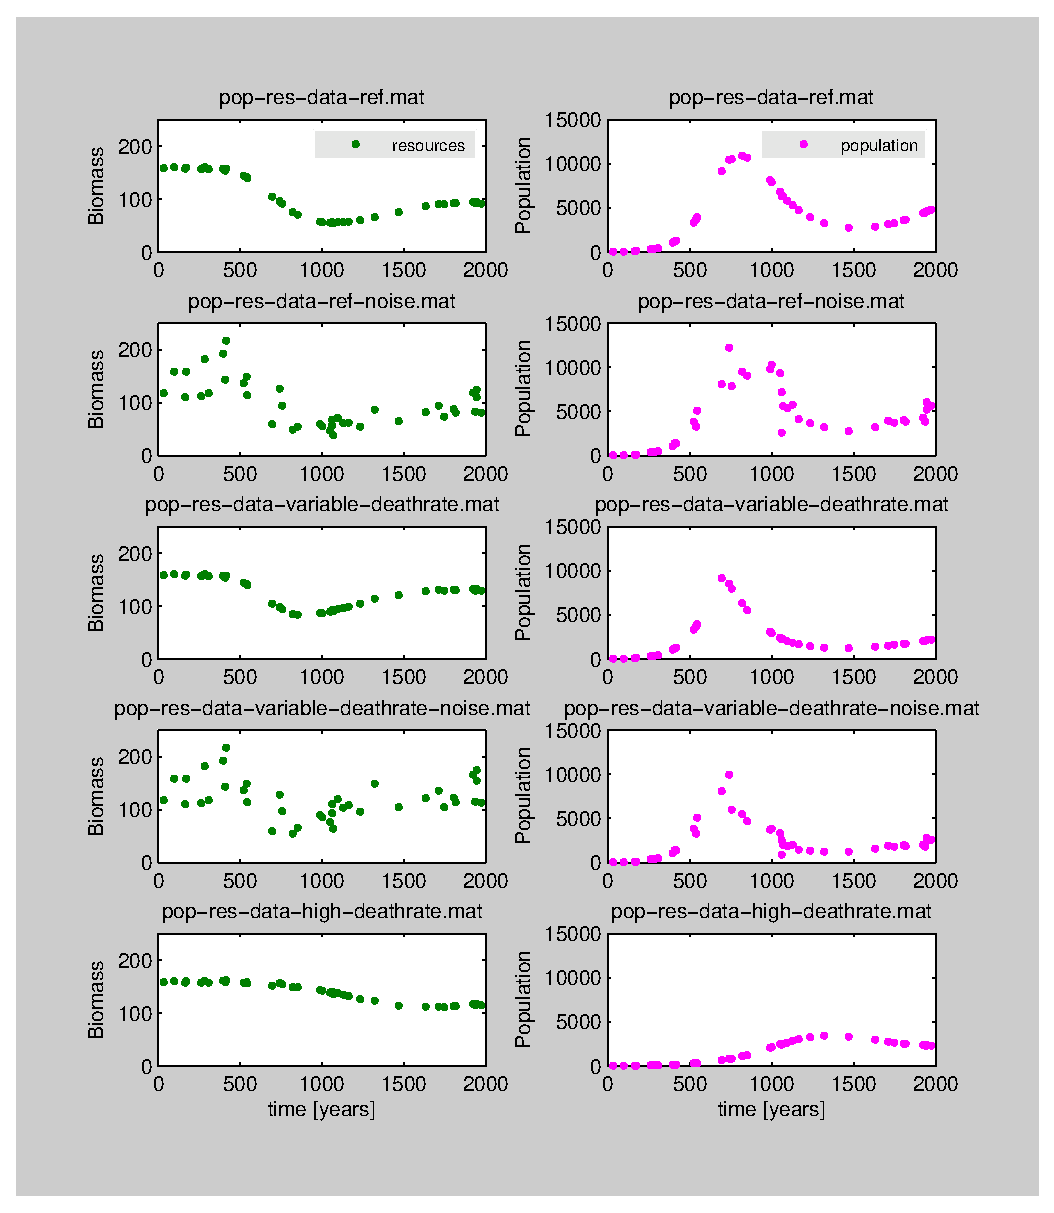
\includegraphics[width=1.0\textwidth]{./eps/converted/pop-res-figures}
  \caption{Resources-Population plots for the various files.}
  \label{fig:pop-res-figures}
\end{figure}



\needspace{15\baselineskip}
So far, we have calibrated the \mcode{eastermodel} based on either Population or Resources, but you could also use both variables simultaneously. To do this, we need to make some changes to the model:

\lstinputlisting[numbers=none,nolol,label={lst:weighted-error-series-modelside}]{./../m/weighted-error-series-modelside.m}

With this code, the model returns an error series, rather than the states themselves, so the objective function should no longer compare model output with observations; instead, we now want to minimize the model output. A simple way to accomplish this is by setting \mcode{Measurement.MeasData} to \mcode{zeros(size(PopMeas))}.

\smallq{Use the MATLAB editor to open `dreamWithEasterModelMO.m' from `./exercises/dream-easter-island-mo/'. Make the appropriate changes to the program in order to use both Population and Resources information. Set \mcode{Extra.popWeight} to 1.0 for now (i.e.~ignoring the misfit on Resources) and don't forget to initialize \mcode{Extra.argOutIsErr} as well. With this weighting factor, your result should be similar to that of a single-objective optimization (when the objective function operates on Population). Run the script. Store your results.}


\smallq{Now do the same thing, but with all weight on the Resources. Again, store the result.}

\smallq{Repeat one more time, but with half the weight on the Population and half the weight on Resources. Store the result. Explain why the last result looks much more like the result of \mcode{Extra.popWeight=1.0} than that of \mcode{Extra.popWeight=0.0}.}

\smallq{How would you make sure that Population and Resources are treated as equally important variables when \mcode{Extra.popWeight=0.5}? Implement your solution and check if there is any difference with your earlier results.}

\smallq{Adapt the script to let it use the Resources data from `pop-res-data-ref.mat' and the Population data from `pop-res-data-high-deathrate.mat' with:
\lstinputlisting[numbers=none,nolol,label={lst:load-selected-variables}]{./../m/load-selected-variables.m}
Run the script for \mcode{Extra.popWeight} equal to 1.0, 0.0, and 0.5. Explain the results.
}%smallq



\smallqo{Looking back at the single-objective exercises that we have done earlier this week, which one do you think would benefit from a multi-objective approach? Explain what variables you would use in the calibration and which objectives you would use (and why) before implementing it.}


\section{Multi-objective optimization of HYMOD}


\smallqo{In the directory `./exercises/hymod-so/' you will find the files to apply the SCE-UA algorithm \citep{duan-gupt-soro1992} to the HYMOD model. We use the same data as in previous exercises (Leaf River, Mississippi), and we analyze the data from a single year (1953). Open `CompOF.m' and verify what objective function is being used in the current optimization. In a first step, compare the root mean square error (RMSE) and the mean absolute error (MAE). Run SCE-UA and save the best parameters and the associated model runs (BestSim and bestSets) for both objective functions. Note that the objection function values for RMSE and MAE are given at the end of the SCE-UA run. Are the optimized parameters different for the two objective functions? Are the model predictions different? Can you understand why?}

\smallqo{If you like, you can implement alternative objective functions. If you need inspiration, you might want to take a look at Table~1 in \citet{gupt-soro-yapo1998}; see the `./papers/' folder. Alternatively, you can apply a Box-Cox transformation to the data. Again, can you understand why the model parameters and model predictions are different? Is one of the optimized parameter sets superior to another one?}

\smallqo{The Pareto front can be approximated by varying the weights $a$ and $b$ in the following objective function: $a*RMSE+b*MAE$. If $a=1$ and $b=0$, you should get the same result as for the single-objective optimization with RMSE as the objective function. Implement this weighted objective function in \mcode{CompOF} and run the SCE-UA algorithm with different selections for the parameters $a$ and $b$. Were you able to systematically explore the Pareto front? Is this an efficient approach?}

\smallqo{In order to explore the Pareto front between the RMSE and the MAE more accurately, we will apply the MOSCEM-UA algorithm to HYMOD. You can find the code in the directory `./exercises/hymod-mo/'. The two objective functions are defined at the end of \mcode{hymod}.}

\smallqo{You can start the algorithm by typing \mcode{runMOSCEM} at the command prompt. Compare the results of MOSCEM-UA with those of the previous exercise. Does MOSCEM-UA provide a good estimate of the Pareto front? Do the optimized parameters vary systematically along the Pareto front? Can you draw any conclusions about the model from this? Explore different objective functions.}





\smallq{Formulate 2 conclusions on the basis of today's activities:
\begin{enumerate}
\item{your most important conclusion;}
\item{a conclusion based on your findings, that you don't expect anyone else has found.}
\end{enumerate}
}%smallq



\backmatter

\bibliographystyle{chicago}
\bibliography{./../bib/literaturedb}


%\printindex
\insertemptypage{}

\end{document}
